\chapter{Unternehmen}
\section{Informationen zum Unternehmen}
Die Firma \textbf{Robot Technology and Innovations GmbH (RTI)} wird im Juli 2018 von vier Akademikern gegründet. Das Unternehmen beschäftigt sich mit der Entwicklung neuartiger Steuerungen, die speziell für industrielle Roboter eingesetzt werden. \\
Die Anteile der Firma wurden zu je 25\% auf die Geschäftsführer- und -innen aufgeteilt. 

%TODO Kooperationspartner, vor -und nachteile von kooperationspartner (ev. Kooperationspartner: F & E Wels?)


\section{Status der Unternehmensgründung}
Auf Grund der Rechtsform müssen wir unsere GmbH ins Firmenbuch eintragen lassen. Die Genehmigung der Gewerbeberechtigung muss noch durch das Magistrat Linz stattgegeben werden. 


\section{Firmensitz}
Der Firmensitz der \textbf{Robot Technology and Innovations GmbH}  befindet sich im Gewerbegebiet in Linz, Franzosenhausweg 49a. Ein Vorteil der Liegenschaft ist die exzellente Verkehrsanbindung, da sich unser Unternehmen gleich in der Nähe der Autobahnabfahrt Linz/Franzosenhausweg befindet. 

\section{Organisationsstruktur}
In Abbildung \ref{fig:organigrammrti} kann man das Organigramm der RTI-GmbH begutachten. 
\begin{figure}[h]
	\centering
	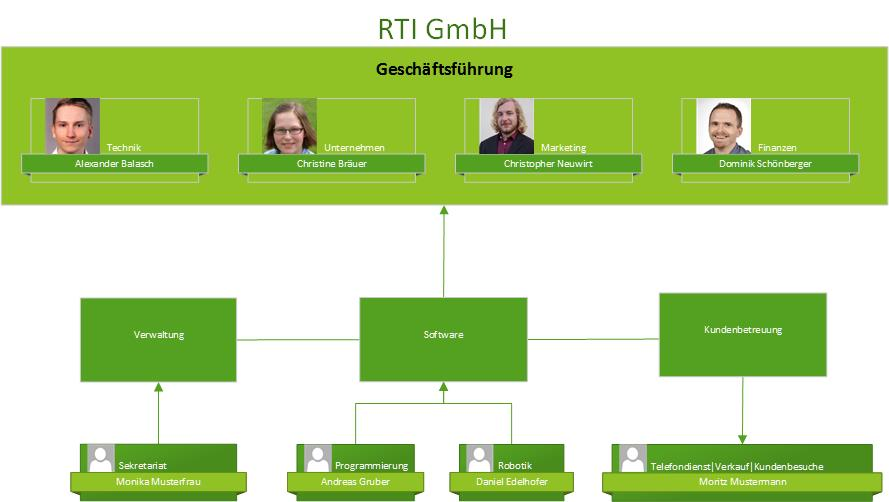
\includegraphics[width=1\linewidth]{Images/OrganigrammRTI}
	\caption{Organigramm der RTI-GmbH}
	\label{fig:organigrammrti}
\end{figure}

\newpage

\section{Ziele}
Durch unsere realistischen Zielsetzungen haben wir ein gemeinsames Bild  im Kopf, was wir in Zukunft erreichen wollen. Zusätzlich haben wir unsere Ziele in kurz-, mittel- und langfristige Ziele eingeteilt. \\ 

\textbf{Kurzfristige Ziele}
\begin{itemize}
	\item Wir wollen einen Gesellschaftsvertrag abschließen, um eine GmbH zu gründen.  % Abschluss des Gesellschaftsvertrages
	\item Erfolgreiche Genehmigung der Gewerbeberechtigung durch das Magistrat Linz. %Genehmigung der Gewerbeberechtigung
	\item Die Formalitäten der Gründung abschließen und danach das Unternehmen ins Firmenbuch eintragen lassen.  %Eintrag ins Firmenbuch
	\item Wir wollen in den ersten zwei Geschäftsjahren Marktführer in der Region werden. %Marktführerschaft in der Region
	\item Durch Veranstaltungen, Messen,... wollen wir neue Geschäftskontakte knüpfen. %Knüpfung von Geschäftskontakten
	\item Nach dem zweiten Geschäftsjahr wollen wir den Break-Even-Point erreicht haben. 
\end{itemize} 

\newpage

\textbf{Mittelfristige Ziele}
\begin{itemize}
	\item Wir wollen nach drei Jahren ein Umsatzwachstum von 40\% gegenüber dem Vorjahr erwirtschaften. %Umsatzwachstum von 40\% gegenüber dem Vorjahr
	\item Das Unternehmen soll um eine eigene Produktions- und Testhalle erweitert werden. %Eigene Testhalle
	\item Nach drei Jahren wollen wir am internationalen Markt teilnehmen. \\ %
\end{itemize}

\textbf{Langfristige Ziele}
\begin{itemize}
	\item Nach fünf Jahren wollen wir zu den Marktführer in der EU gehören.  %Marktführerschaft in der EU
	\item Ebenfalls nach fünf Jahren wollen wir einen weiteren Standort eröffnen. %Ausbau des Standortes
	\item Nach sechs Jahren wollen wir einen soliden Mitarbeiterstamm von 50 Personen aufweisen. \\%Mitarbeiterzuwachs
\end{itemize}

\section{Gründungsteam}
\textbf{Alexander Balasch, BSc. Geschäftsführer} \\
Alexander absolviert gerade den Diplomstudiengang Automatisierungstechnik an der FH Oberösterreich, Campus Wels, welchen er voraussichtlich im Juli 2018 abschließen wird. Den darauf aufbauenden Bachelorstudiengang absolvierte er an der FH Oberösterreich im Fachbereich Automatisierungstechnik. Zuvor besuchte er die HTL-Wels, Schwerpunkt Maschinenbau, und leistete seinen Zivildienst. Während der Schullaufbahn und des Studiums absolvierte er Praktika bei den Firmen Rübig und Plasser\&Theurer, sowie der TGW und hat somit bereits Erfahrung in der praktische Umsetzung von Projekten im Softwarebereich. 

\textbf{Christine Bräuer, BSc. Geschäftsführerin} \\
Christine absolviert gerade den Diplomstudiengang Automatisierungstechnik an der FH Oberösterreich, Campus Wels, welchen sie voraussichtlich im September 2018 abschließen wird. Den Bachelorstudiengang absolvierte sie an der FH Oberösterreich, Campus Hagenberg in Medizin- und Bioinformatik. 
Neben ihrer schulischen Laufbahn ist sie seit 2010 Schriftführerin-Stv. und seit 2016 auch im Organisationsteam des Blasorchesters St. Valentin Steyr-Traktoren tätig, wo sie ihre organisatorischen Fähigkeiten und ihr Engagement ausgebaut hat. Seit 2014 arbeitet sie nebenberuflich regelmäßig bei den BMW Werken in Steyr, wo sie schon einige Erfahrung in den Bereichen Produktion und Fertigung als auch in der Montage sammeln konnte. \\

\newpage

\textbf{Christopher Neuwirt, BSc. Geschäftsführer} \\
Christopher absolviert gerade den Diplomstudiengang Automatisierungstechnik an der FH Oberösterreich, Campus Wels, welchen er voraussichtlich im September 2018 abschließen wird. Den zugehörigen Bachelorstudiengang absolvierte er mit gutem Erfolg ebenfalls an der FH Oberösterreich. Nach Abschluss der HTL Paul-Hahn-Straße in Linz, höhere Abteilung für Mechatronik, begann er nach einem halben Jahr als Angebotszeichner bei Rosenbauer International sein Studium. Während dieser Zeit eignete er sich Erfahrung in den Bereichen Projektmanagement und Konstruktion an. Seit 2016 arbeitete er zuerst als Praktikant und später Teilzeit bei B\&R Industrial Automotion und war dort in der Lage sich tiefergreifendes Wissen über Steuerungen, Sicherheitstechnik als auch Inverter zur Motorensteuerung anzueignen.\\

\textbf{Ing. Dominik Schönberger, BSc. Geschäftsführer} \\
Dominik absolviert gerade den Diplomstudiengang Automatisierungstechnik an der FH Oberösterreich, Campus Wels, welchen er voraussichtlich im Juli 2018 abschließen wird. Den Bacholorstudiengang Automatisierungstechnik am Campus Wels schloss er mit ausgezeichnetem Erfolg ab.  Nach dem Abschluss der HTL Neufelden, Schwerpunkt Automatisierungstechnik, war Dominik als Systems Engineer bei der TGW Mechanics GmbH in Wels tätig. Dort konnte er sich Wissen im Bereich Projektmanagment, Produktion, Konstruktion und Systemplanung aneignen. Ausbildung von neuen Mitarbeitern und Führung von kleinen Projektteams zählten ebenfalls zu seinen Tätigkeiten. 2011/2012 war Dominik als technischer Leiter in Dänemark und fungierte während dieser Zeit als stellvertretender Projektmanager vor Ort.\\

\subsection{Bisherige Zusammenarbeit}
Alexander, Christopher und Dominik haben drei Jahre gemeinsam an der FH Wels studiert und haben sich durch viele gemeinsame Projekte besser kennengelernt. Seit einem Jahr studieren wir alle vier gemeinsam an der FH Wels und fungieren bei einigen Projekten als zusammengehöriges Projektteam. Wir haben gleiche Ziele vor Augen und ziehen immer gemeinsam an einem Strang. 


\subsection{Erfahrungen und Fähigkeiten des Gründerteams}
Die nachfolgenden Abbildungen \ref{tab: Hard Skills des Gründerteams} \& \ref{tab: Soft Skills des Gründerteams} zeigen unsere Erfahrungen und Fähigkeiten, aber auch welche Kompetenzlücken wir durch andere Mitarbeiter noch schließen müssen. \\
\newpage
In Abbildung \ref{tab: Hard Skills des Gründerteams} lautet die Legende wie folgt: 
\begin{itemize}
	\item 1 = sehr gute Kenntnisse
	\item 2 = gute Kenntnisse
	\item 3 = Grundkenntnisse
	\item 4 = keine Kenntnisse \\\\ 
\end{itemize}

%TODO Tabellenbeschriftung, Legende für Kenntnisse (1 = sehr gute Kenntnisse, 2 = gute Kenntnisse, 3 = Grundkenntnisse, 4 = keine Kenntnisse)
\begin{table}[h]
\begin{tabular}{|>{\centering\arraybackslash}p{3cm}|>{\centering\arraybackslash}p{2.5cm}|>{\centering\arraybackslash}p{2.5cm}|>{\centering\arraybackslash}p{2.5cm}|>{\centering\arraybackslash}p{2.5cm}|}
	\hline 
	Gründerteam & {Alexander Balasch} & Christine Bräuer & Christopher Neuwirt & Dominik Schönberger \\ 
	\hline 
	\multicolumn{5}{|c|}{Hard Skills} \\ 
	\hline
	Finanzen \& Controlling 		& 2 & 2 & 4 & 3 \\ 
	\hline 
	Fremdsprachen 					&  3 & 2 & 2 & 2 \\
	\hline
	Marketing 						& 3 & 4 & 3 & 4 \\ 
	\hline 
	Software \& Hardware 			& 1 & 1 & 2 & 2 \\ 
	\hline 	
	Organisations- fähigkeit 		& 2  & 1 & 2 & 2 \\ 
	\hline	
	Personalwesen \& Entwicklung 	& 3 & 3 & 3 & 3 \\
	\hline
	Produktion 						& 3 & 3 & 3 & 2 \\
	\hline
	Projekt- management 			& 3 & 3 & 2 & 1 \\ 
	\hline 
	Verkauf 						& 2 & 4 & 3 & 2 \\ 
	\hline
\end{tabular}
\caption{Hard Skills des Gründerteams}
\label{tab: Hard Skills des Gründerteams} 
\end{table}

Für Abbildung \ref{tab: Soft Skills des Gründerteams} lautet die Legende wie folgt: 
\begin{itemize}
	\item 1 = Fähigkeit, Erfahrung sehr gut ausgeprägt
	\item 2 = Fähigkeit, Erfahrung gut ausgeprägt
	\item 3 = grundsätzliche Erfahrung vorhanden
	\item 4 = keine Erfahrung
\end{itemize}
%TODO Tabellenbeschriftung, Legende für Kenntnisse (1 = Fähigkeit, Erfahrung sehr gut ausgeprägt, 2= gut ausgeprägt, 3= grundsätzliche Erfahrung vorhanden, 4 = keine Erfahrung)
\begin{table}[h]
\begin{tabular}{|>{\centering\arraybackslash}p{3cm}|>{\centering\arraybackslash}p{2.5cm}|>{\centering\arraybackslash}p{2.5cm}|>{\centering\arraybackslash}p{2.5cm}|>{\centering\arraybackslash}p{2.5cm}|}
	\hline 
	Gründerteam & Alexander Balasch & Christine Bräuer & Christopher Neuwirt & Dominik Schönberger \\ 
	\hline 
	\multicolumn{5}{|c|}{Soft Skills} \\ 
	\hline 
	Anpassungs- fähigkeit 		& 2 & 2 & 2 & 2 \\ 
	\hline 
	Belastbarkeit 				& 1 & 1 & 1 & 1 \\ 
	\hline 
	Charisma 					& 2 & 2 & 1 & 2 \\ 
	\hline 
	Durchsetzungs- vermögen 	& 2 & 2 & 2 & 1 \\ 
	\hline 
	Engagement  				& 1 & 1 & 1 & 1 \\  %und Einsatzbereitschaft
	\hline 
	Empathie					& 2 & 2 & 1 & 3 \\ 
	\hline 
	Flexibilität 				& 2 & 1 & 2 & 2 \\ 
	\hline 
	Kommunikations- fähigkeit 	& 1 & 2 & 1 & 2 \\ 
	\hline 
	Kritikfähigkeit 			& 1 & 2 & 2 & 1 \\ 
	\hline  
	Konflikt- fähigkeit 		& 2 & 2 & 3 & 1 \\ 
	\hline 
	Kunden- orientierung 		& 1 & 2 & 2 & 2 \\ 
	\hline 
	Menschen- kenntnis 			& 1 & 2 & 1 & 2 \\ 
	\hline 
	Motivation 					& 1 & 1 & 1 & 1 \\ 
	\hline 
	Präsentations- stärke 		& 1 & 2 & 1 & 2 \\ 
	\hline  
	Teamfähigkeit 				& 1 & 2 & 1 & 2 \\ 
	\hline 
	Urteilsvermögen 			& 2 & 1 & 2 & 2 \\ 
	\hline 
	Verhandlungs- kompetenz		& 1 & 2 & 2 & 2 \\ 
	\hline 
	Verantwortung 				& 1 & 1 & 1 & 1 \\ 
	\hline 
	Zeitmanagement 				& 1 & 1 & 3 & 2 \\ 
	\hline 
	Zielorientierung 			& 1 & 1 & 1 & 1 \\ 
	\hline 
\end{tabular} 
\caption{Soft Skills des Gründerteams}
\label{tab: Soft Skills des Gründerteams}
\end{table}

\newpage
\section{Mitarbeiter in der Start-Up Phase (bis Ende 2019)}
Für die Start-Up Phase werden folgende Mitarbeiter eingestellt. \\\\
\textbf{Festangestellte Mitarbeiter}
\begin{itemize}
	\item 1 Mitarbeiterin im Bereich Sekretariat
	\item 1 Mitarbeiter im Bereich Programmierung
	\item 1 Mitarbeiter im Bereich Robotik
	\item 1 Mitarbeiter im Bereich des Kundendienstes 
\end{itemize}
